%\documentclass[tikz]{standalone}
%\usepackage{polyglossia} %configuración de idioma
\setmainlanguage{spanish} %elegir idioma español
\usepackage{fontspec} %paquete para cargar fuentes
\setsansfont{cmunb}[Extension=.otf,
UprightFont=*mr,
ItalicFont=*mo,
BoldFont=*sr, % semibold
BoldItalicFont=*so, % semibold oblique
NFSSFamily=cmbr
]
\usepackage{cmbright} %fuentes
\usepackage{microtype} %mejorar generales al documento pdf
\usepackage{amsmath} %paquete matemáticos
\usepackage{amsfonts} %fuentes matemáticas varias
\usepackage{amssymb} %símbolos matemáticos varios
\documentclass[../../master.tex]{subfiles}
\begin{document}
    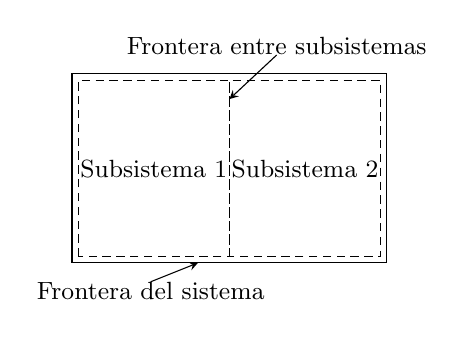
\begin{tikzpicture}[scale=0.8]
        \draw (-2.5,-1.5) rectangle (2.5,1.5); %sistema
        \draw[densely dashed] (-2.4,-1.4) rectangle node[midway] {\small Subsistema 1} (0,1.4); %subsistema 1
        \draw[densely dashed] (0,-1.4) rectangle node[midway] {\small Subsistema 2} (2.4,1.4); %subsistema 2
        \draw[-stealth] (-1.25,-1.8) -- (-0.5, -1.5); %Flecha para la frontera del subsistema
        \node at (-1.25, -1.95) {\small Frontera del sistema}; %Label para la frontera del sistema
        \draw[-stealth] (0.75,1.8) -- (0,1.1); %Linea para la frontera entre subsistemas
        \node at (0.75,1.95) {\small Frontera entre subsistemas}; %Label de la frontera entre sistemas
        \draw[draw=none] (-2.8,-1.5) rectangle (2.8,1.5); %Delimitador de imagen
    \end{tikzpicture}
\end{document}
